\documentclass[SE,authoryear,toc]{lsstdoc}
% lsstdoc documentation: https://lsst-texmf.lsst.io/lsstdoc.html
\input{meta}

% Package imports go here.

% Local commands go here.

%If you want glossaries
%\input{aglossary.tex}
%\makeglossaries

\title{Working with Rubin EFD timestamps.}

% Optional subtitle
% \setDocSubtitle{A subtitle}

\author{%
Craig Lage
}

\setDocRef{SITCOMTN-018}
\setDocUpstreamLocation{\url{https://github.com/lsst-sitcom/sitcomtn-018}}

\date{\vcsDate}

% Optional: name of the document's curator
\setDocCurator{Craig Lage}

\setDocAbstract{%
There are some subtleties to working with the timestamps in the EFD, and how they relate to the FITS file header keywords.  This technote attempts to capture my learning on this topic.
}

% Change history defined here.
% Order: oldest first.
% Fields: VERSION, DATE, DESCRIPTION, OWNER NAME.
% See LPM-51 for version number policy.
\setDocChangeRecord{%
  \addtohist{1}{YYYY-MM-DD}{Unreleased.}{Craig Lage}
}


\begin{document}

% Create the title page.
\maketitle
% Frequently for a technote we do not want a title page  uncomment this to remove the title page and changelog.
% use \mkshorttitle to remove the extra pages

% ADD CONTENT HERE

\section{Introduction}

I have been working with the timestamps in the Rubin EFD (Engineering Facilities Database), and have generated some notebooks and learning that is captured in this technote.  This also relates to the timestamps in the generated FITS file headers.  This work is with the Auxiliary Telescope, but it is believed that it will translate to ComCam and LSSTCam files as well.

\section{UTC vs TAI}

There are two important time scales to remember, UTC and TAI.  A simple introduction to these can be found at the following Wikipedia pages:
\begin{enumerate}
  \item \url{https://en.wikipedia.org/wiki/Coordinated_Universal_Time}
  \item \url{https://en.wikipedia.org/wiki/International_Atomic_Time}
\end{enumerate}

From the point of view of this technote, the following things are important to remember:
\begin{enumerate}
  \item UTC is the time reported by any Unix computer, and is typically what is used as a timebase in any commercially available software.
  \item UTC has one second discontinuties in the past whenever a ``leap-second'' was applied to keep the UTC timebase in sync with the Earth's rotation.  There may be further discontinuties in the future if a leap second is added or subtracted.
  \item TAI is a continuous time base without these discontinuties.
  \item Because of the accumulated leap seconds, TAI is currently exactly 37 seconds ahead of UTC.  
\end{enumerate}

\section{Timestamps in the EFD}

There are two types of time information in the EFD:
\begin{enumerate}
  \item Event time stamps that are updated once per second.  An example of one of these is ``lsst.sal.ATMCS.logevent\_allAxesInPosition''
  \item Events that need to be sampled more often, such as the position of the mount.  An example of one of these is ``lsst.sal.ATMCS.mount\_AzEl\_Encoders''.  For these events, every second 100 values are entered into the EFD, indicating the position of the mount every 10 milliseconds for the preceding second.  These are indexed from 0-99, and are called ``packed time series''.  These is software (lsst\_efd\_client.merge\_packed\_time\_series) that parses these packed time series and returns a pandas dataframe with the sequential measurements.
\end{enumerate}

\section{Example notebook to query these times.}

I have generated a simple notebook to illustrate accessing these times from the FITS headers and from the EFD.  It is for a single exposure on the AuxTel on 04-Aug-2021.  I will attempt to keep this notebook (and this document) up to date as things change.  Thenotebook can be accessed in two places:
\begin{enumerate}
  \item \url{https://github.com/craiglagegit/ScratchStuff/blob/master/notebooks/Plot_Tracking_3_13Aug21.ipynb}
  \item At NCSA at /project/cslage/AuxTel/notebooks/Plot\_Tracking\_3\_13Aug21.ipynb
\end{enumerate}

The graph generated by this notebook is shown below.  It shows the mount tracking, then a small adjustment was made to center the image (at about 02:07:44), then the ``allAxesInPosition'' time stamp is received at about 02:07:46, then the exposure is taken between about 02:07:56 and 02:07:58.

  \begin {figure} {H}
    \centering
    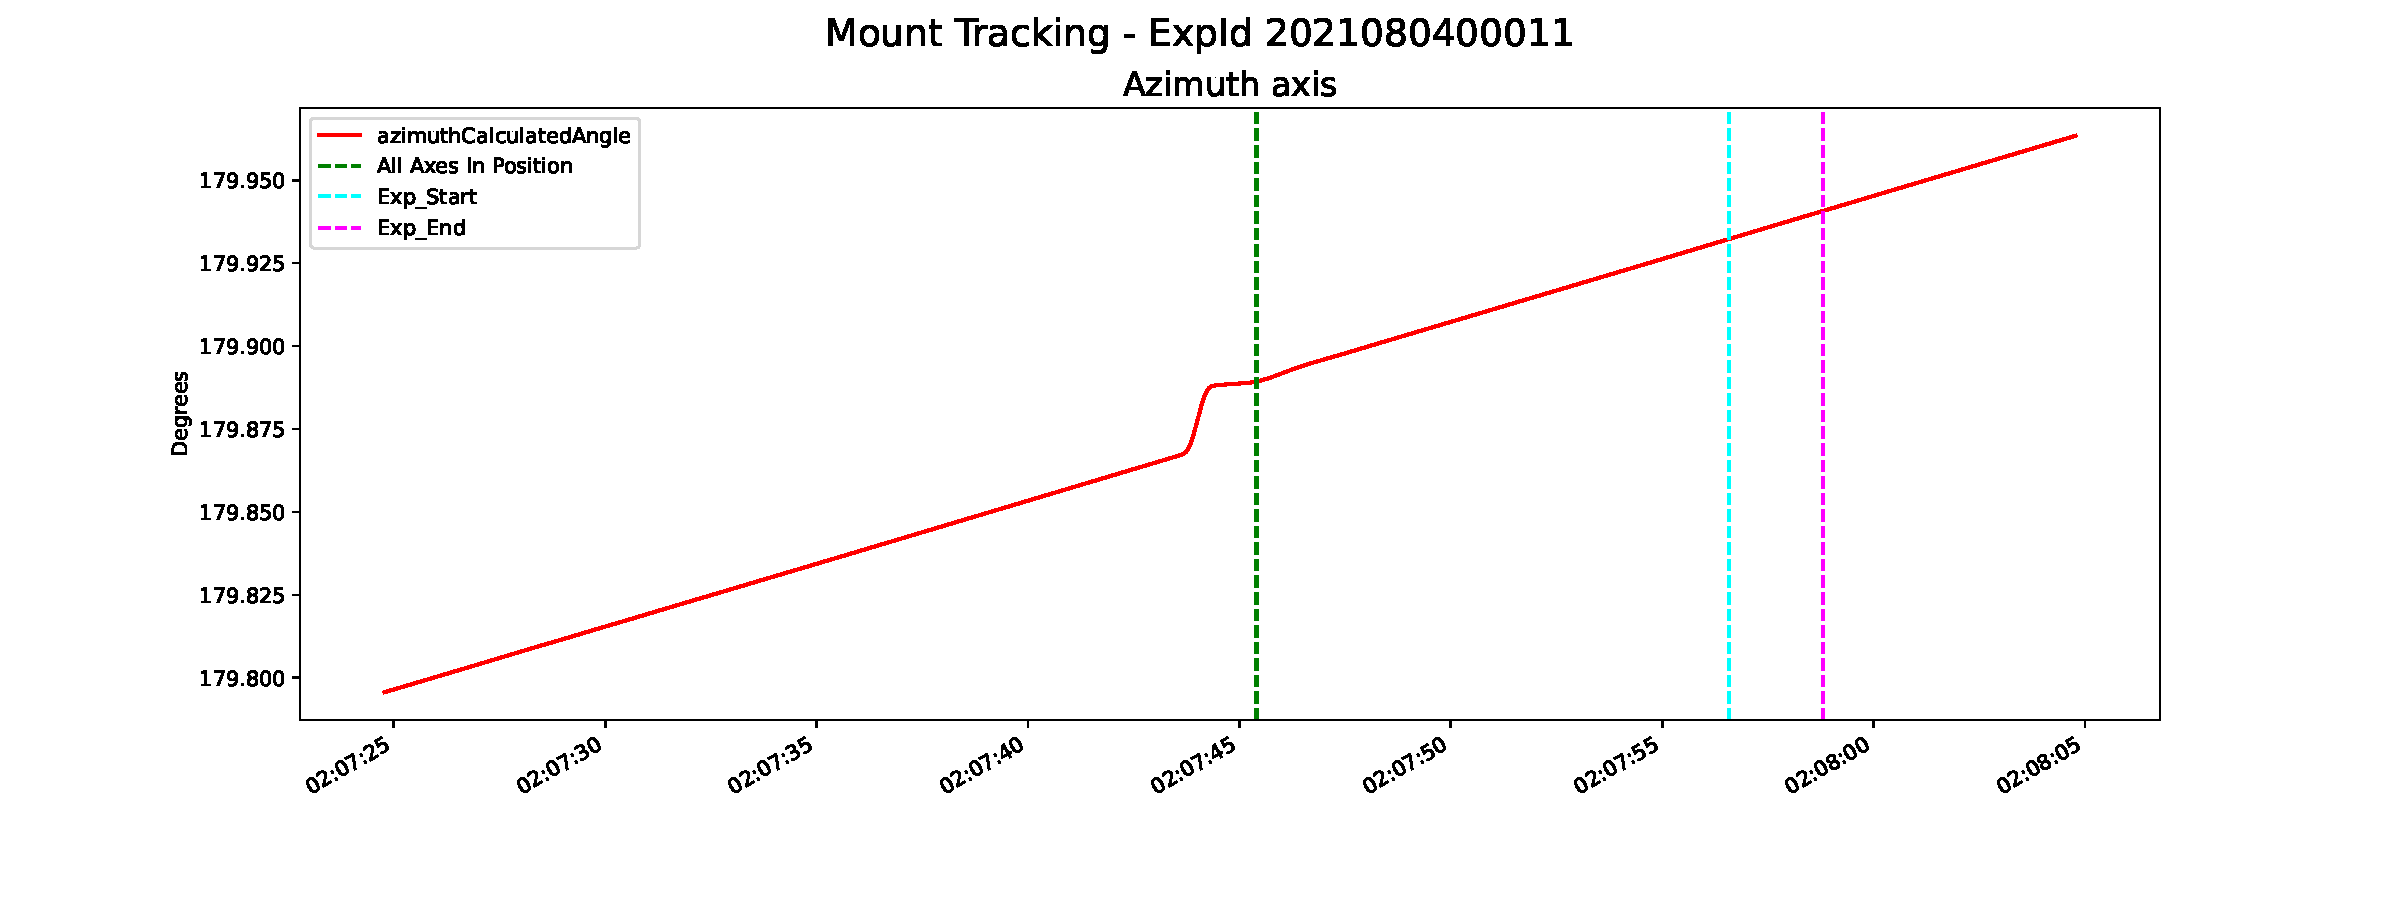
\includegraphics[trim=0.0in 0.0in 0.0in 0.0in,clip,width=0.99\textwidth]{Tracking_Timebase_2021080400011_13Aug21.pdf}
  % Trim is Left Bottom Right Top
  \end{figure}

\section{Important things to remember}

There are several pieces of learning that came out of this exercise:
\begin{enumerate}
  \item In the FITS headers, The DATE-BEG and DATE-END keywords represent the time of shutter open and close, and are in TAI, as specified by the TIMESYS keyword.  The DATE keyword is the time the file was written, and is in UTC, as specified by the FITS specification.
  \item Pandas indicates that the timestamps in the EFD are in UTC, but this is not correct.  All of the timestamps in the EFD should be in TAI.
    \item When using lsst\_efd\_client.merge\_packed\_time\_series, you currently need to override the default (internal\_time\_scale="tai"), and specify (internal\_time\_scale="utc").  I am unclear as to the resolution of this, but it has been reported that this is an astropy bug that is being worked on.
\end{enumerate}



% You can also use the \input command to include several content files.

\appendix
% Include all the relevant bib files.
% https://lsst-texmf.lsst.io/lsstdoc.html#bibliographies
\section{References} \label{sec:bib}
\renewcommand{\refname}{} % Suppress default Bibliography section
\bibliography{local,lsst,lsst-dm,refs_ads,refs,books}

% Make sure lsst-texmf/bin/generateAcronyms.py is in your path
\section{Acronyms} \label{sec:acronyms}
\addtocounter{table}{-1}
\begin{longtable}{p{0.145\textwidth}p{0.8\textwidth}}\hline
\textbf{Acronym} & \textbf{Description}  \\\hline

ComCam & The commissioning camera is a single-raft, 9-CCD camera that will be installed in LSST during commissioning, before the final camera is ready. \\\hline
EFD & Engineering and Facility Database \\\hline
FITS & Flexible Image Transport System \\\hline
LSST & Legacy Survey of Space and Time (formerly Large Synoptic Survey Telescope) \\\hline
NCSA & National Center for Supercomputing Applications \\\hline
SE & System Engineering \\\hline
TAI & International Atomic Time \\\hline
UTC & Coordinated Universal Time \\\hline
\end{longtable}

% If you want glossary uncomment below -- comment out the two lines above
%\printglossaries





\end{document}
